\documentclass[lecture,12pt,]{pcms-l}
\input preamble.tex
\input header.tex

%%%%%%%%%%%%%%%%%%%%%%%%%%%%%%%%%%%%%%%%%%%%%%%%%%%%%%%%%%%%%

\begin{document}
\mainmatter
\setcounter{page}{1}

\lectureseries[\course]{\course}

\auth[R.A. de Callafon]{Lecturer: \lecAuth\\ Scribe: \scribe}
\date{November 5, 2009}

\setaddress

% the following hack starts the lecture numbering at 15
\setcounter{lecture}{20}
\setcounter{chapter}{20}

\lecture{Midterm Notes}

\section{2006-2d/2007-1d}
For the unweighted parameter estimate $\hat{\theta}_N$ is given by
$$\hat{\theta}_N = \left[\frac{1}{N}\sum_{t=1}^N\vp(t)\vp^T(t)\right]^{-1}\left[\frac{1}{N}\sum_{t=1}^N\vp(t)y(t)\right]$$
To prove that the cross-correlation function $\hat{R}_{\epsilon u}^N(\tau)$ between prediction error $\epsilon(t,\hat{\theta}_N)$ and input $u(t)$ satisfies $\hat{R}_{\epsilon u}^N(\tau)=0$ for $\tau=0,1,\ldots,n$ we have to know that
\begin{itemize}
\item $u\perp e$
\item $E\{e(t)u(t-\tau)\}=0$
\item $\lim_{N\to\infty}\hat{R}_{eu}^N(\tau))=0$. This one we can never compute.
\end{itemize}
All of those items are equivalent. Suppose we get ``white noise'' inputs and error in \textsc{Matlab} using \texttt{e=randn(N,1)} and \texttt{u=randn(N,1)}. Is $\hat{R}_{eu}(\tau)=0 ~\forall \tau$? Not in \textsc{Matlab} because the randomness is finite. At some point the random sequence will begin to repeat.

However, notice that the LS estimate gives the prediction error as $\epsilon(t)=y(t)-\vp^T(t)\hat{\theta}_{LS}^N$. This means that $\hat{R}_{\epsilon u}^N(\tau)=0$ for $\tau=1,\ldots,n$, where $n$ is the number of past inputs in $\vp(t)$. This is true because of the way the LS estimate is constructed as an orthogonal projection of the output $y(t)$ onto the space of $\vp^T(t)\theta$ while letting $\theta$ vary. See Figure \ref{fig:mt062d2}. This guarantees that $\epsilon(t)$ is orthogonal to $\vp^T(t)$ which contains the past inputs and outputs. Since the prediction error is orthogonal to the past ($n$) inputs the cross-correlation is zero. See Figure \ref{fig:mt062d1}.

\begin{figure}[ht!]
  \centering
  \includegraphics[width=.5\textwidth]{images/mt062d2}
  \caption{Projection of output $y(t)$ onto space of $\vp^T(t)\theta$ with $\theta$ varying. Shows projection error.}
  \label{fig:mt062d2}
\end{figure}

\begin{figure}[ht!]
  \centering
  \includegraphics[width=.5\textwidth]{images/mt062d1}
  \caption{Cross-correlation function between noise error and input, prediction error and input.}
  \label{fig:mt062d1}
\end{figure}

We can also see this from the equation
$$\sum\vp(t)y(t) = \sum\vp(t)\vp^T(t)\underbrace{\theta}_{LS} + \underbrace{\sum\vp(t)\epsilon(t)}_{=0, \vp\perp\epsilon}$$


\end{document}

%%%%%%%%%%%%%%%%%%%%%%%%%%%%%%%%%%%%%%%%%%%%%%%%%%%%%%%%%%%%%